%\title{LaTeX Portrait Poster Template}
%%%%%%%%%%%%%%%%%%%%%%%%%%%%%%%%%%%%%%%%%
% a0poster Portrait Poster
% LaTeX Template
% Version 1.0 (22/06/13)
%
% The a0poster class was created by:
% Gerlinde Kettl and Matthias Weiser (tex@kettl.de)
% 
% This template has been downloaded from:
% http://www.LaTeXTemplates.com
%
% License:
% CC BY-NC-SA 3.0 (http://creativecommons.org/licenses/by-nc-sa/3.0/)
%
%%%%%%%%%%%%%%%%%%%%%%%%%%%%%%%%%%%%%%%%%

%----------------------------------------------------------------------------------------
%	PACKAGES AND OTHER DOCUMENT CONFIGURATIONS
%----------------------------------------------------------------------------------------
\documentclass[a0,portrait]{a0poster}
\usepackage{multicol} % This is so we can have multiple columns of text side-by-side
\columnsep=100pt % This is the amount of white space between the columns in the poster
\columnseprule=3pt % This is the thickness of the black line between the columns in the poster

\usepackage[svgnames]{xcolor} % Specify colors by their 'svgnames', for a full list of all colors available see here: http://www.latextemplates.com/svgnames-colors

\usepackage{times} % Use the times font
%\usepackage{palatino} % Uncomment to use the Palatino font

\usepackage{graphicx} % Required for including images
\graphicspath{{figures/}} % Location of the graphics files
\usepackage{booktabs} % Top and bottom rules for table
\usepackage[font=normalsize,labelfont=bf]{caption} % Required for specifying captions to tables and figures
\usepackage{amsfonts, amsmath, amsthm, amssymb} % For math fonts, symbols and environments
\usepackage{wrapfig} % Allows wrapping text around tables and figures
\usepackage{natbib}

\begin{document}

%----------------------------------------------------------------------------------------
%	POSTER HEADER 
%----------------------------------------------------------------------------------------

% The header is divided into two boxes:
% The first is 75% wide and houses the title, subtitle, names, university/organization and contact information
% The second is 25% wide and houses a logo for your university/organization or a photo of you
% The widths of these boxes can be easily edited to accommodate your content as you see fit
%
\begin{minipage}[b]{0.15\textwidth}

\includegraphics[width=10cm]{cornkey.png}\\
%
\includegraphics[width=5cm]{pslogo.jpg}\\
\end{minipage}
%
\begin{minipage}[b]{0.7\textwidth}
\Huge \color{NavyBlue} \textbf{Utilizing Evolutionary Conservation Information to \\ Improve Prediction Accuracy in Genomic Selection} \color{Black}\\[1cm] % Title
%\Huge\textit{An Exploration of Complexity}\\[2cm] % Subtitle
\Large \textbf{Jinliang Yang$^1$, Sofiane Mezmouk$^{1,2}$, Rita Mumm$^3$, and Jeffrey Ross-Ibarra$^1$ }\\[0.5cm] % Author(s)
\large $^1$Department of Plant Sciences, University of California, Davis, CA 95616, USA \\%[0.4cm] % University/organization
\large $^2$Current address: KWS SAAT AG, Grimsehlstr. 31, 37555 Einbeck, Germany \\ %[0.4cm] % University/organization
\large $^3$Department of Crop Sciences, University of Illinois at Urbana-Champaign, Urbana, IL 61801, USA \\[0.4cm] % University/organization
%\Large \texttt{john@LaTeXTemplates.com} --- 1 (000) 111 1111\\
\end{minipage}
%
\begin{minipage}[b]{0.15\textwidth}

\includegraphics[width=10cm]{pslogo.jpg}\\
\end{minipage}
%


\vspace{1cm} % A bit of extra whitespace between the header and poster content

%----------------------------------------------------------------------------------------

\begin{multicols}{2} % This is how many columns your poster will be broken into, a portrait poster is generally split into 2 columns

%----------------------------------------------------------------------------------------
%	ABSTRACT
%----------------------------------------------------------------------------------------

\color{Navy} % Navy color for the abstract

\section*{ABSTRACT}
Genomic selection (GS) has gained popularity recently as the availability of genome-wide markers has increased. Current methods for GS weigh all the available SNPs equally in model training, without considering their functional differences. Genetic variations detected at evolutionary conserved sites tend to be deleterious and, thus, may be more informative for GS. To utilize this kind of information as a prior into the GS model, we proposed a method to put more weight on evolutionarily constrained sites. As a proof-of-concept, a half diallel population based on 12 diverse inbred lines was used, from which seven phenotypic traits were collected. Some of these traits show high levels of heterosis. After sequencing the 12 founder lines, about 14 million SNPs were discovered and the SNPs were used to identify 502,913 haplotype blocks shared through identity by descent (IBD). A five fold cross-validation experiment was conducted using the summary statistics of the SNP conservation scores, which were computed by evaluating sequences similarity of multiple divergent species, in the IBD blocks as explanatory variables. The results show that the prediction accuracies are significantly better than shuffled data with randomly assigned conservation scores. This study demonstrates the importance of incorporating evolutionary information in GS and its potential use in plant breeding.


%----------------------------------------------------------------------------------------
%	INTRODUCTION
%----------------------------------------------------------------------------------------

\color{SaddleBrown} % SaddleBrown color for the introduction

\section*{Objectives}
\begin{itemize}
\item Study deleterious variants in a maize diallel population and their contributions to heterosis.
\item Quantify IBD blocks by using evolutionary conservation information.
\item Test whether it is useful to incorporate evolutionary conservation information in genomic selection.
\end{itemize}

%----------------------------------------------------------------------------------------
%	MATERIALS AND METHODS
%----------------------------------------------------------------------------------------

\section*{Materials and Methods}

\subsection*{Plant material and phenotypic data}
%-------------------
%Figure
\begin{center}\vspace{1cm}
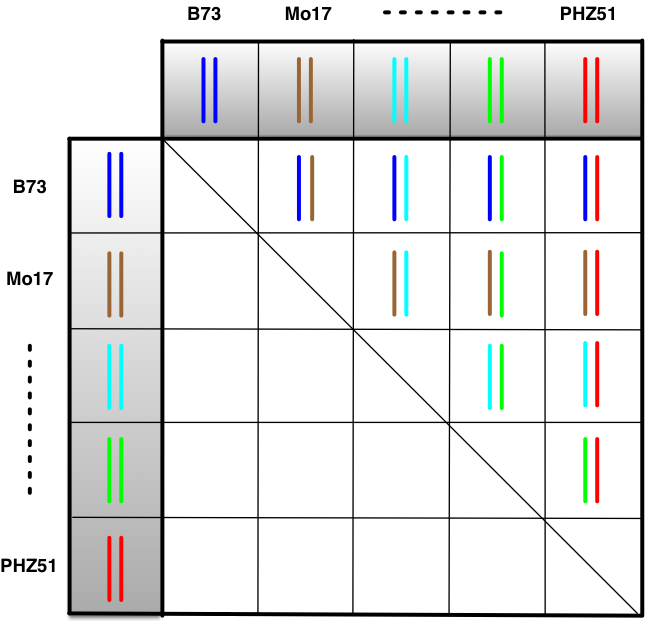
\includegraphics[width=0.8\linewidth]{pvp.pdf}
\captionof{figure}
{\color{black} \textbf{Diallel experimental design and distribution of phenotypic data.}
(A) Twelve maize inbred lines were selected and crossed in a partial diallel fashion without considering reciprocal effects. Ten of these inbreds (LH1, LH123HT, LH82, PH207, 4676A, PHG39, PHG47, PHG84, PHJ40, PHZ51) are proprietary inbreds that have expired from Plant Variety Protection (PVP) and represent the lineage of key heterotic germplasm pools used in present-day commercial corn hybrids. And two of them are predominant public inbreds, B73 and Mo17. (B) Phenotypic data were collected for anthesis-silking interval (ASI, in days), days to 50\% pollen shed (DTP), days to 50\% silking (DTS), ear height (EHT, in cm), grain yield adjusted to 15.5\% moisture (GY, in bu/A), plant height (PHT, in cm), and test weight (TW, in pounds).
}
\end{center}\vspace{1cm}

\subsection*{Sequencing and SNP conservation annotation}
%------------------
% wet lab
The DNAs from twelve inbred lines were isolated and sequenced to an average coverage of 10X. Read pairs kept after filtering were mapped to the maize B73 reference genome (AGPv2) with bwa-mem. Reads, with mapping quality (MAPQ) higher than 10 and with a best alignment score higher than the second best one, were kept for further analyses. After filtering, 13,782,809 were kept for further comparisons, including 1,909,416 genic SNPs and 361,280 in protein coding regions. Genome-wide deleterious variants were characterized by using genomic evolutionary rate profiling (GERP) \citep{Davydov2010}. For each position after multiple alignment, GERP scores were obtained by computing the regected substitutions subtracted by the neutral rate in a set of sequenced plant genomes. 

\begin{center}\vspace{1cm}
\includegraphics[width=0.8\linewidth]{gerp.pdf}
\captionof{figure}{
\color{black} \textbf{Conservation scores distribution of diallel SNPs and relationship between GERP and minor allele frequency.}
(A) Among the $\sim$14 million SNPs identified in the diallel population, $\sim$1.2 million ($\sim$10\%) sites could obtain their evolutionary conservation information using GERP. Of these sites, 506,898 (42\%) are evolutionary constraint; variants at these sites were considered as deleterious.  
(B) Mean GERP scores were calculated for each bin (bin size = 0.01) of minor allele frequency (MAF). The regression analysis indicated that variants at conserved sites tend to be maintained in a low frequency. Red line denotes regression line and grey lines define its 95\% confidence interval.}
\end{center}\vspace{1cm}

%Figure GERP IBD
\subsection*{Computing conservation score for IBD blocks}
%------------------

\begin{center}\vspace{1cm}
\includegraphics[width=1\linewidth]{gerpIBD.pdf}
\captionof{figure}{
\color{black} \textbf{Incoporation of conservation information into IBD blocks.}
The SNPs in a IBD block were added up with their GERP scores as the conservation estimates, which were calculated with both additive and dominant models. Under the additive model, 2 x GERP score was assigned to the homozygous loci with non-reference SNP calls, 1 x GERP score was assigned to the heterozygous loci, and 0 was assigned to the homozygous loci with reference SNP calls. Under the dominant model, 1 x GERP score was assigned to both the homozygous loci with non-reference SNP calls and heterozygous loci, 0 was assigned to homozygous loci with reference SNP calls.}
\end{center}\vspace{1cm}

%----------------------------------------------------------------------------------------
%	RESULTS 
%----------------------------------------------------------------------------------------

\section*{Results}

A haplotype based genomic selection strategy was conceived by using conservation scores of the IBD blocks as the explanatory variables. SNP loci with GERP score $>$0 were considered as evolutionary conserved sites, and genomic variations detected at these sites were treated as deleterious. A Bayesian-based approach (BayesC) \citep{} was employed for the GS experiments. To rule out the possibility that prediction taking advantage of the more informative genic SNPs, the same set of genic SNPs were used for real and circular shuffled experiments.

As a result, we found that for the trait per se, the prediction accuracies were singificantly improved for ASI, DTS and PHT with the additive model. Prediction accuracies were significantly improved for ASI, DTP, GY and TW with the dominant model. In general, the average prediction rates are higher using additive model (r = 0.8) than dominant model (r = 0.7). For the heterosis transformation traits, for example, percent high parental heterosis (pHPH), only one prediction rate was significantly increased for the GY pHPH. 

\begin{center}\vspace{1cm}
\includegraphics[width=0.8\linewidth]{cvres.pdf}
\captionof{figure}{
\color{black} \textbf{Beanplots of the cross-validation accuracies.}
The cross-validation experiments were conducted using genic SNPs and circular shuffled data from the same set of the genic SNPs for trait per se with additive model (A), trait per se with dominant model (B), pHPH with the additive model (C) and pHPH with the dominant model (D). Accuaries drived from the real data were plotted on the left side of the bean (blue) and accuracies derived from the circular shuffled data were plotted on the right side of the bean (grey). Horizotal bars on beans indicate the mean accuracies. Grey dashed line indicate overall average. Stars on top of the beans indicate significantly improved cross-validation accuracies.
}
\end{center}\vspace{1cm}

%----------------------------------------------------------------------------------------
%	CONCLUSIONS
%----------------------------------------------------------------------------------------

\color{SaddleBrown} % SaddleBrown color for the conclusions to make them stand out

\section*{Conclusions}

\begin{itemize}
\item Large number (N=506,898) of deleterious alleles were identified in elite maize lines. The GERP enabled us to identify deleterious alleles beyond the protein coding region.
\item A genomic selection pipeline was developed, which utilized evolutionary conservation information in the model.
\item Cross-validation results suggested the prediction accuracies could be significantly improved for some of the traits with additive and dominant models. 


\end{itemize}

\color{DarkSlateGray} % Set the color back to DarkSlateGray for the rest of the content

%----------------------------------------------------------------------------------------
%	FORTHCOMING RESEARCH
%----------------------------------------------------------------------------------------

%\section*{Forthcoming Research}



%----------------------------------------------------------------------------------------
%	REFERENCES
%----------------------------------------------------------------------------------------

%\nocite{*} % Print all references regardless of whether they were cited in the poster or not
\bibliographystyle{plain} % Plain referencing style
\bibliography{sample} % Use the example bibliography file sample.bib

%----------------------------------------------------------------------------------------
%	ACKNOWLEDGEMENTS
%----------------------------------------------------------------------------------------

\section*{Acknowledgements}

Thanks for the funding!

%----------------------------------------------------------------------------------------

\end{multicols}
\end{document}